\begin{block}{Tracing}
  \begin{center}
    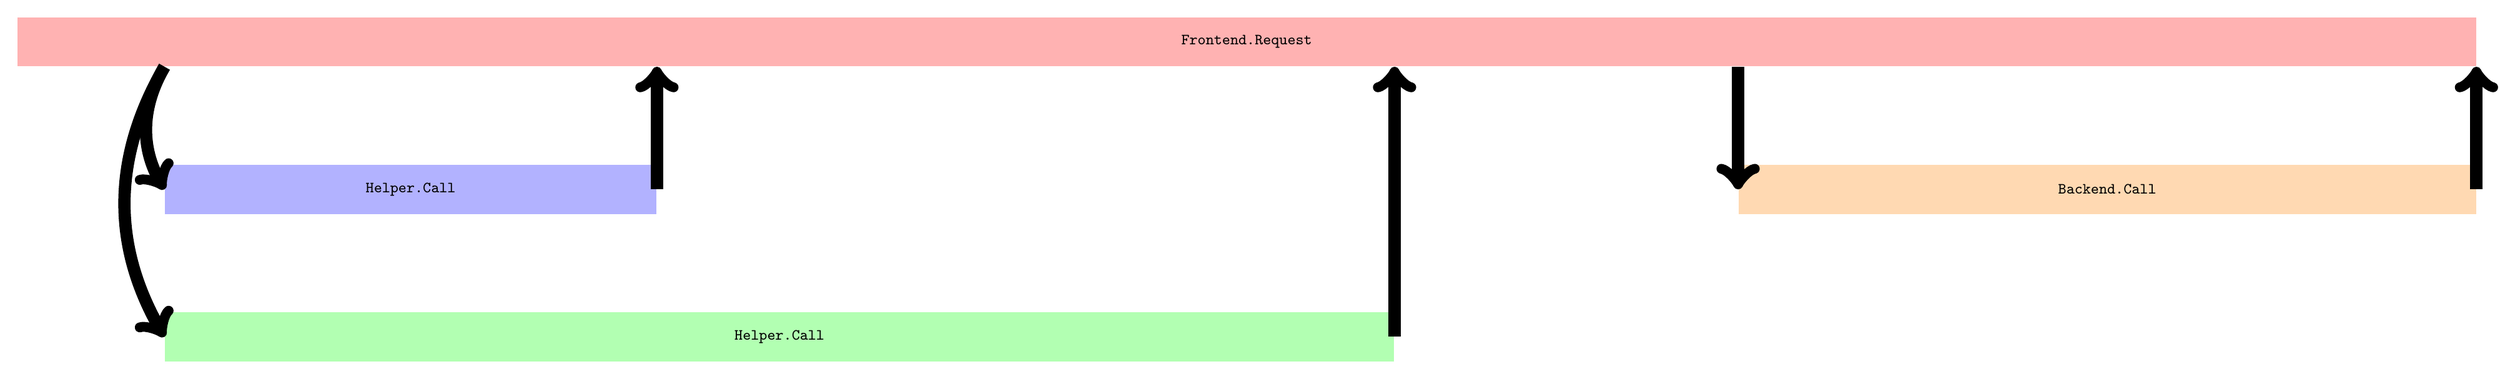
\begin{tikzpicture}
      \ttfamily
      \small
      \tikzstyle{event}=[minimum height=1cm, anchor=west]
      \tikzstyle{arrow}=[line width=0.25 cm, ->]
      \node[event, fill=red!30,    minimum width=50cm] (a) at (0,  6) {Frontend.Request};
      \node[event, fill=blue!30,   minimum width=10cm] (b) at (3,  3) {Helper.Call};
      \node[event, fill=green!30,  minimum width=25cm] (c) at (3,  0) {Helper.Call};
      \node[event, fill=orange!30, minimum width=15cm] (d) at (35, 3) {Backend.Call};

      \draw[arrow] (a.south -| b.west) to[bend right] (b.west);
      \draw[arrow] (a.south -| c.west) to[bend right] (c.west);
      \draw[arrow] (b.east) to (a.south -| b.east);
      \draw[arrow] (c.east) to (a.south -| c.east);
      \draw[arrow] (a.south -| d.west) to (d.west);
      \draw[arrow] (d.east) to (a.south -| d.east);
    \end{tikzpicture}
  \end{center}

  \vspace{3cm}

  \begin{center}
    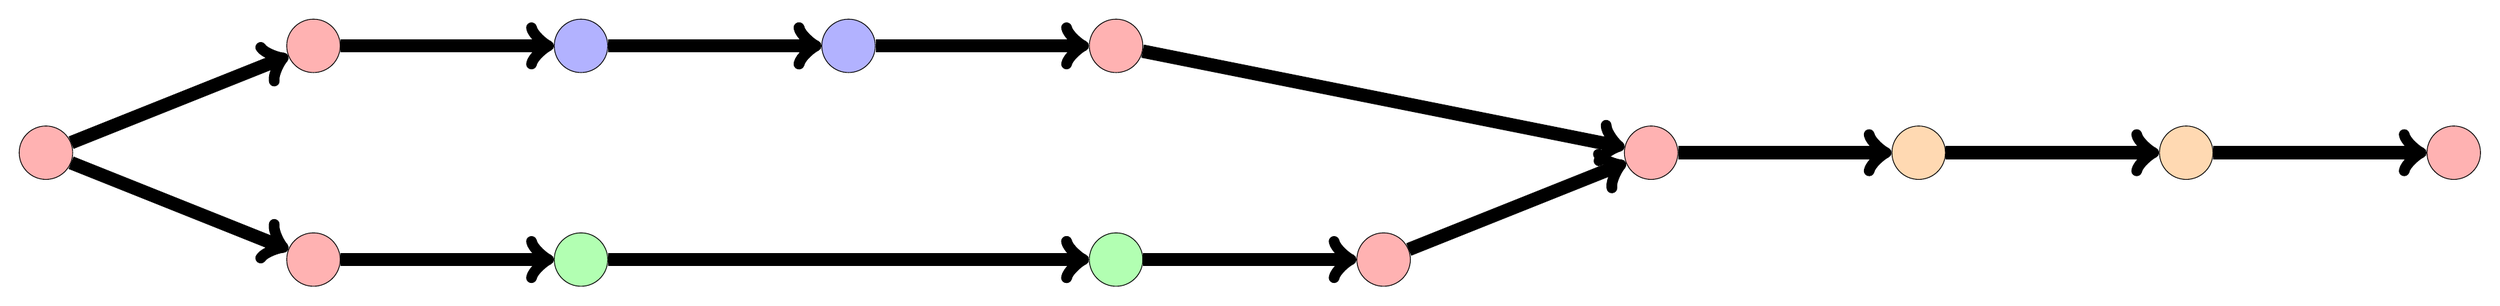
\begin{tikzpicture}[yscale=2, xscale=5]
      \tikzstyle{tup}=[draw, shape=circle, minimum width=1cm]
      \tikzstyle{arrow}=[line width=0.25 cm, ->]
      \tikzstyle{a}=[fill=red!30]
      \tikzstyle{b}=[fill=blue!30]
      \tikzstyle{c}=[fill=green!30]
      \tikzstyle{d}=[fill=orange!30]
      \node[tup, a] (a1) at (0, 1) {};
      \node[tup, a] (ab) at (1, 2) {};
      \node[tup, a] (ac) at (1, 0) {};
      \node[tup, b] (b1) at (2, 2) {};
      \node[tup, b] (b2) at (3, 2) {};
      \node[tup, c] (c1) at (2, 0) {};
      \node[tup, c] (c2) at (4, 0) {};
      \node[tup, a] (ba) at (4, 2) {};
      \node[tup, a] (ca) at (5, 0) {};
      \node[tup, a] (a2) at (6, 1) {};
      \node[tup, d] (d1) at (7, 1) {};
      \node[tup, d] (d2) at (8, 1) {};
      \node[tup, a] (a3) at (9, 1) {};

      \foreach \src/\dst in {a1/ab, ab/b1, b1/b2, b1/b2, b2/ba, ba/a2, a1/ac,
                             ac/c1, c1/c2, c1/c2, c2/ca, ca/a2, a2/d1, d1/d2,
                             d2/a3} {%
        \draw[arrow] (\src) to (\dst);
      }
    \end{tikzpicture}
  \end{center}
\end{block}
